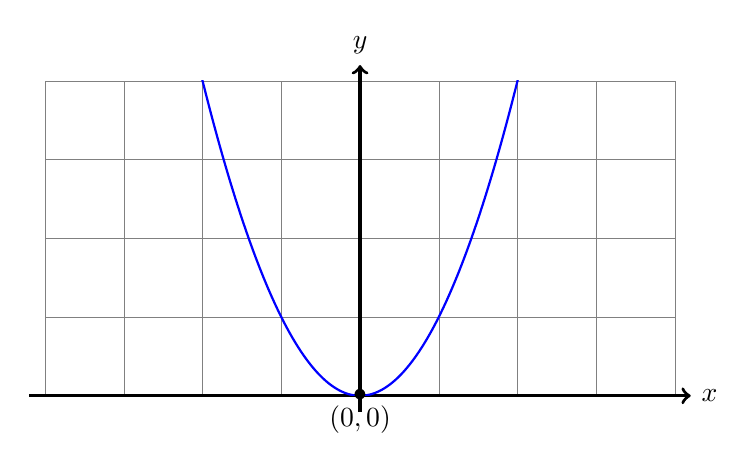
\begin{tikzpicture}
  \draw[very thin,color=gray] (-4,0) grid (4,4);

  \draw[very thick,->] (-4.2,0) -- (4.2,0) node[right] {$x$};
  \draw[very thick,->] (0,-0.2) -- (0,4.2) node[above] {$y$};

  \begin{scope}
    \clip (-4,0) rectangle (4,4);
    \draw [color=blue,thick] plot[smooth,samples=500] (\x,{(\x)^2});
  \end{scope}

  \node at (0,0) {$\bullet$};
  \node [below] at (0,0) {$(0,0)$};

\end{tikzpicture}
